% Template for PLoS
% Version 3.0 December 2014
%
% To compile to pdf, run:
% latex plos.template
% bibtex plos.template
% latex plos.template
% latex plos.template
% dvipdf plos.template
%
% % % % % % % % % % % % % % % % % % % % % %
%
% -- IMPORTANT NOTE
%
% This template contains comments intended
% to minimize problems and delays during our production
% process. Please follow the template instructions
% whenever possible.
%
% % % % % % % % % % % % % % % % % % % % % % %
%
% Once your paper is accepted for publication,
% PLEASE REMOVE ALL TRACKED CHANGES in this file and leave only
% the final text of your manuscript.
%
% There are no restrictions on package use within the LaTeX files except that
% no packages listed in the template may be deleted.
%
% Please do not include colors or graphics in the text.
%
% Please do not create a heading level below \subsection. For 3rd level headings, use \paragraph{}.
%
% % % % % % % % % % % % % % % % % % % % % % %
%
% -- FIGURES AND TABLES
%
% Please include tables/figure captions directly after the paragraph where they are first cited in the text.
%
% DO NOT INCLUDE GRAPHICS IN YOUR MANUSCRIPT
% - Figures should be uploaded separately from your manuscript file.
% - Figures generated using LaTeX should be extracted and removed from the PDF before submission.
% - Figures containing multiple panels/subfigures must be combined into one image file before submission.
% See http://www.plosone.org/static/figureGuidelines for PLOS figure guidelines.
%
% Tables should be cell-based and may not contain:
% - tabs/spacing/line breaks within cells to alter layout or alignment
% - vertically-merged cells (no tabular environments within tabular environments, do not use \multirow)
% - colors, shading, or graphic objects
% See http://www.plosone.org/static/figureGuidelines#tables for table guidelines.
%
% For tables that exceed the width of the text column, use the adjustwidth environment as illustrated in the example table in text below.
%
% % % % % % % % % % % % % % % % % % % % % % % %
%
% -- EQUATIONS, MATH SYMBOLS, SUBSCRIPTS, AND SUPERSCRIPTS
%
% IMPORTANT
% Below are a few tips to help format your equations and other special characters according to our specifications. For more tips to help reduce the possibility of formatting errors during conversion, please see our LaTeX guidelines at http://www.plosone.org/static/latexGuidelines
%
% Please be sure to include all portions of an equation in the math environment.
%
% Do not include text that is not math in the math environment. For example, CO2 will be CO\textsubscript{2}.
%
% Please add line breaks to long display equations when possible in order to fit size of the column.
%
% For inline equations, please do not include punctuation (commas, etc) within the math environment unless this is part of the equation.
%
% % % % % % % % % % % % % % % % % % % % % % % %
%
% Please contact latex@plos.org with any questions.
%
% % % % % % % % % % % % % % % % % % % % % % % %

\documentclass[10pt,letterpaper]{article}
\usepackage[top=0.85in,left=2.75in,footskip=0.75in]{geometry}

% Use adjustwidth environment to exceed column width (see example table in text)
\usepackage{changepage}

% Use Unicode characters when possible
\usepackage[utf8]{inputenc}

% textcomp package and marvosym package for additional characters
\usepackage{textcomp,marvosym}

% fixltx2e package for \textsubscript
\usepackage{fixltx2e}

% amsmath and amssymb packages, useful for mathematical formulas and symbols
\usepackage{amsmath,amssymb}

% cite package, to clean up citations in the main text. Do not remove.
\usepackage{cite}
\usepackage[dvipdfm]{hyperref}

% Use nameref to cite supporting information files (see Supporting Information section for more info)
\usepackage{nameref,hyperref}

% line numbers
\usepackage[right]{lineno}

% ligatures disabled
\usepackage{microtype}
\DisableLigatures[f]{encoding = *, family = * }

% rotating package for sideways tables
\usepackage{rotating}

% Remove comment for double spacing
%\usepackage{setspace}
%\doublespacing

\usepackage{algorithm}
\usepackage{algorithmicx}
\usepackage{algpseudocode}
\newcommand{\algorithmicbreak}{\textbf{break}}
\newcommand{\BREAK}{\State \algorithmicbreak}

% Text layout
\raggedright
\setlength{\parindent}{0.5cm}
\textwidth 5.25in
\textheight 8.75in

% Bold the 'Figure #' in the caption and separate it from the title/caption with a period
% Captions will be left justified
\usepackage[aboveskip=1pt,labelfont=bf,labelsep=period,justification=raggedright,singlelinecheck=off]{caption}

% Use the PLoS provided BiBTeX style
\bibliographystyle{plos2009}

% Remove brackets from numbering in List of References
\makeatletter
\renewcommand{\@biblabel}[1]{\quad#1.}
\makeatother

% Leave date blank
\date{}

% Header and Footer with logo
\usepackage{lastpage,fancyhdr,graphicx}
\pagestyle{myheadings}
\pagestyle{fancy}
\fancyhf{}
\lhead{
\includegraphics[natwidth=1.3in,natheight=0.4in]{PLOSlogo.png}}
\rfoot{\thepage/\pageref{LastPage}}
\renewcommand{\footrule}{\hrule height 2pt \vspace{2mm}}
\fancyheadoffset[L]{2.25in}
\fancyfootoffset[L]{2.25in}
\lfoot{\sf PLOS}

%% Include all macros below

\newcommand{\lorem}{{\bf LOREM}}
\newcommand{\ipsum}{{\bf IPSUM}}

%% END MACROS SECTION


\begin{document}
\vspace*{0.35in}

% Title must be 150 characters or less
\begin{flushleft}
{\Large
\textbf\newline{Exploiting Publication Contents and Collaboration Networks for Collaborator Recommendation}
}
\newline
% Insert Author names, affiliations and corresponding author email.
\\
Xiangjie Kong\textsuperscript{1},
Huizhen Jiang\textsuperscript{1},
Haifeng Liu\textsuperscript{1},
Zhen Chen\textsuperscript{1},
Zhenzhen Xu\textsuperscript{1*},
Feng Xia\textsuperscript{1},
Amr Tolba\textsuperscript{2,3}

%Name1 Surname\textsuperscript{1},
%Name2 Surname\textsuperscript{2,\textpilcrow},
%Name3 Surname\textsuperscript{2,\textcurrency a},
%Name4 Surname\textsuperscript{2,\ddag},
%Name5 Surname\textsuperscript{2,\ddag},
%Name6 Surname\textsuperscript{2,\Yinyang},
%Name7 Surname\textsuperscript{3,*,\Yinyang}

\bf{1} School of Software, Dalian University of Technology, China\\
\bf{2} Riyadh Community College, King Saud University, Saudi Arabia\\
\bf{3} Mathematics and Computer Science Department, Faculty of Science, Menoufia University, Egypt
\\
%\bf{2} Affiliation Dept/Program/Center, Institution Name, City, State, Country
%\\
%\bf{3} Affiliation Dept/Program/Center, Institution Name, City, State, Country
%\\

% Insert additional author notes using the symbols described below. Insert symbol callouts after author names as necessary.
%
% Remove or comment out the author notes below if they aren't used.
%
% Primary Equal Contribution Note
%\Yinyang These authors contributed equally to this work.

% Additional Equal Contribution Note
%\ddag These authors also contributed equally to this work.

% Current address notes
%\textcurrency a Insert current address of first author with an address update
% \textcurrency b Insert current address of second author with an address update
% \textcurrency c Insert current address of third author with an address update

% Deceased author note
%\dag Deceased

% Group/Consortium Author Note
%\textpilcrow Insert Collaborative Author line here

* Corresponding author; E-mail: xzz@dlut.edu.cn (ZX)
\end{flushleft}

% Please keep the abstract below 300 words
\section*{Abstract}
Thanks to the proliferation of online social networks, it has become conventional for researchers to communicate and collaborate with each other. Meanwhile, one critical challenge arises, that is, how to find the most relevant and potential collaborators for each researcher? In this work, we propose a novel collaborator recommendation model called CCRec, which combines the information on researchers' publications and collaboration network to generate better recommendation. In order to effectively identify the most potential collaborators for researchers, we adopt a topic clustering model to identify the academic domains, as well as a random walk model to compute researchers' feature vectors. Using DBLP datasets, we conduct benchmarking experiments to examine the performance of CCRec. The experimental results show that CCRec outperforms other state-of-the-art methods in terms of precision, recall and F1 score.


% Please keep the Author Summary between 150 and 200 words
% Use first person. PLOS ONE authors please skip this step.
% Author Summary not valid for PLOS ONE submissions.
%\section*{Author Summary}

\linenumbers

% =============================================================================
\section*{Introduction}
% =============================================================================
The current scale of the Internet has risen beyond the imagination of people due to its rapid development. Consequently, how to obtain useful and effective information has become a complex task as a result of information overload. Recommender systems and techniques reduce the problems and immensely help people by providing easier access to the relevant resources they really need.

Collaboration among researchers often occurs and it has been shown that research collaboration has impact on scientific productivity~\cite{lee2005impact}. Therefore, collaboration recommendation becomes very necessary and has been attracting more and more researchers in recent years. Generally, collaboration recommendation can be grouped into two classes: 1) to recommend the most potential collaborators (MPCs) who have never collaborated with the target (i.e. to build new collaborations); 2) to recommend the most valuable collaborators (MVCs) who have ever collaborated with the target before (i.e. to reinforce old collaborations). Lopes et al.~\cite{lopes2010collaboration} worked on identifying new partners to execute joint research and enhancing the collaboration of current partners for researchers. Chen et al.~\cite{chen2009make} proposed that the purpose of friends recommendation is to make new friends and keep the old. Research on enterprise social networking~\cite{dimicco2008motivations} shows that users in a corporate context are interested in discovering valuable contacts not yet known to them, or connecting to weak ties, in addition to staying in touch with their close colleagues. Our previous work~\cite{li2014acrec,xia2014mvcwalker} focuses on recommending MVCs for researchers and enhancing the collaboration with colleagues in their academic social networks. In this work, in contrast, CCRec has an aptitude for discovering new collaborators with high similarity (i.e. MPCs recommendation).

Considering the inherent requirements, a variety of methods related to collaborators recommendation have been proposed, which involve three main aspects: content-based, social network-based and hybrid recommendation. Some traditional content-based methods extract researchers' academic features through tags of interests, user profiles, publications, etc. Gollapalli et al.~\cite{gollapalli2012similar} proposed models for computing the similarity between researchers based on expertise profiles extracted from their publications and academic home pages. Lopes et al.~\cite{lopes2010collaboration} considered researchers' publications area and the vector space model to make collaboration recommendation. Kim et al.~\cite{kim2010collaborative} proposed a collaborative filtering method to provide an enhanced recommendation quality derived from user-created tags. However, researchers often behave differently across multiple domains of interests, which might introduce topic drift problems in general recommendation systems~\cite{tang2012cross}. Furthermore, a researcher often shows bias on various academic domains. Such behaviors usually reveal academic features of researchers in different domains. Thus, it is imperative to consider academic domains when recommending collaborators.

Ma et al.~\cite{ma2011recommender} analyzed how social network information can benefit recommender systems and proposed a method of improving the performance of recommender systems by incorporating social network information. Huynh et al.~\cite{huynh2013trend} proposed a method based on a combination of probability theory and graph theory for modeling and analysing co-author networks. They explored similar vertices of potential candidates for collaboration recommendation. Their main contribution involves taking the trend information into considering when computing the similarity of vertices. Many other approaches~\cite{chen2012discovering,sun2011co} have been presented to formalize academic collaboration recommendation as a link prediction problem in social networks. Some of these approaches have been applied to large social networks and the relevant results show good performance. Lichtenwalter et al.~\cite{lichtenwalter2010new} examined some important factors for link prediction and proposed a general framework, in addition to our previous work~\cite{li2014acrec,xia2014mvcwalker}. Besides, in our previous work we proposed two social network-based models respectively called ACRec~\cite{li2014acrec} and MVCWalker~\cite{xia2014mvcwalker}, both of which solved the problem of recommending MVCs. ACRec enables the collaborated researchers to collaborate with each other again. However, many scientists also initiate collaborations outside of their social networks. It is burdensome and fraught with risk of initiating collaboration with socially unconnected researchers. Therefore, unconnected researchers (MPCs) might be valuable to be recommended.

Some hybrid collaboration recommendation models have been introduced in recent years. Lee et al.~\cite{lee2011recommending} exploited how well content-based, social network-based and hybrid recommendation algorithms predict coauthor relationship. The given results show that a hybrid algorithm combining content and social networks information performs better. Some other brilliant hybrid algorithms can be found in e.g. \cite{cohen2013recommending}, ~\cite{petertonkoker2014scientific} and ~\cite{xia2014socially}. Recently, Chaiwanarom et al.~\cite{chaiwanarom2014collaborator} proposed a new hybrid algorithm for recommending appropriate collaborators in interdisciplinary computer science using degrees of collaborative forces, temporal evolution of research interest, and comparative seniority status. The result shows that it is effective and innovative. However, there are also some issues concerning the recommendation in other research fields besides computer science. Chen et al.~\cite{chen2011collabseer} discussed CollabSeer, an open system to recommend potential research collaborators for researchers and scientists. They discovered collaborators based on the structure of coauthor networks and the user's topic of research interests. This previous work, along with e.g. ~\cite{li2014author}, stimulated our inspiration to introduce a topic model in CCRec.

Here we propose a novel hybrid model by exploiting publication contents and collaboration networks for collaborators recommendation (CCRec). In summary, we make the following contributions in this paper: 1) To compute the most potential collaborators recommendation, we develop a model CCRec, which combines the content-based and social network-based methods. By adopting this procedure, our approach is more favourable in terms of achieving remarkable personalized collaborators recommendation. 2) To reveal researchers' academic features in different domains, we present the feature vectors by utilizing a topic clustering model and a random walk model. 3) We conduct extensive experiments on a subset of DBLP data set to evaluate the performance of CCRec in various scenarios. Moreover, we measured our previous ACRec model and the common neighbors-based model (CNRec) for comparison. Promising results are presented and analyzed.


% =============================================================================
\section*{Methods}
% =============================================================================
Our proposed recommendation scheme for CCRec is inspired by the reality and truth that a researcher usually desires to know other researchers who have similar research interests and strong influence in academia. As mentioned above, researchers often behave differently across multiple domains of interests. Such behaviors usually reveal the academic features of researchers in different domains. Besides, as a social-based model, Random Walk with Restart recommendation model (RWR) has been proved to be competent for calculating the rank score of nodes in social networks derived from co-authorship~\cite{li2014acrec}. Researchers' strength of influence in specific domains can be well reflected by RWR. In this work, we first adopt a content-based method to acquire multiple domains of interests. Secondly, we employ the social network-based method of RWR to measure the researchers' strength of influence in different domains. In the final step of our design, we use the feature vector to evaluate the similarity of researchers and then obtain the recommendation list. The detailed process is described below and the corresponding pseudo-code is illustrated in \nameref{Algorithm1}. Figure~\ref{Fig. 1} depicts the three main components of CCRec.

\begin{figure}[!hbt]
\caption{{\bf The architecture of CCRec.} Depicts the three main components of CCRec: topic clustering and researcher partition, random walk, similarity calculation and top-N recommendation.}
\label{Fig. 1}
%\center
%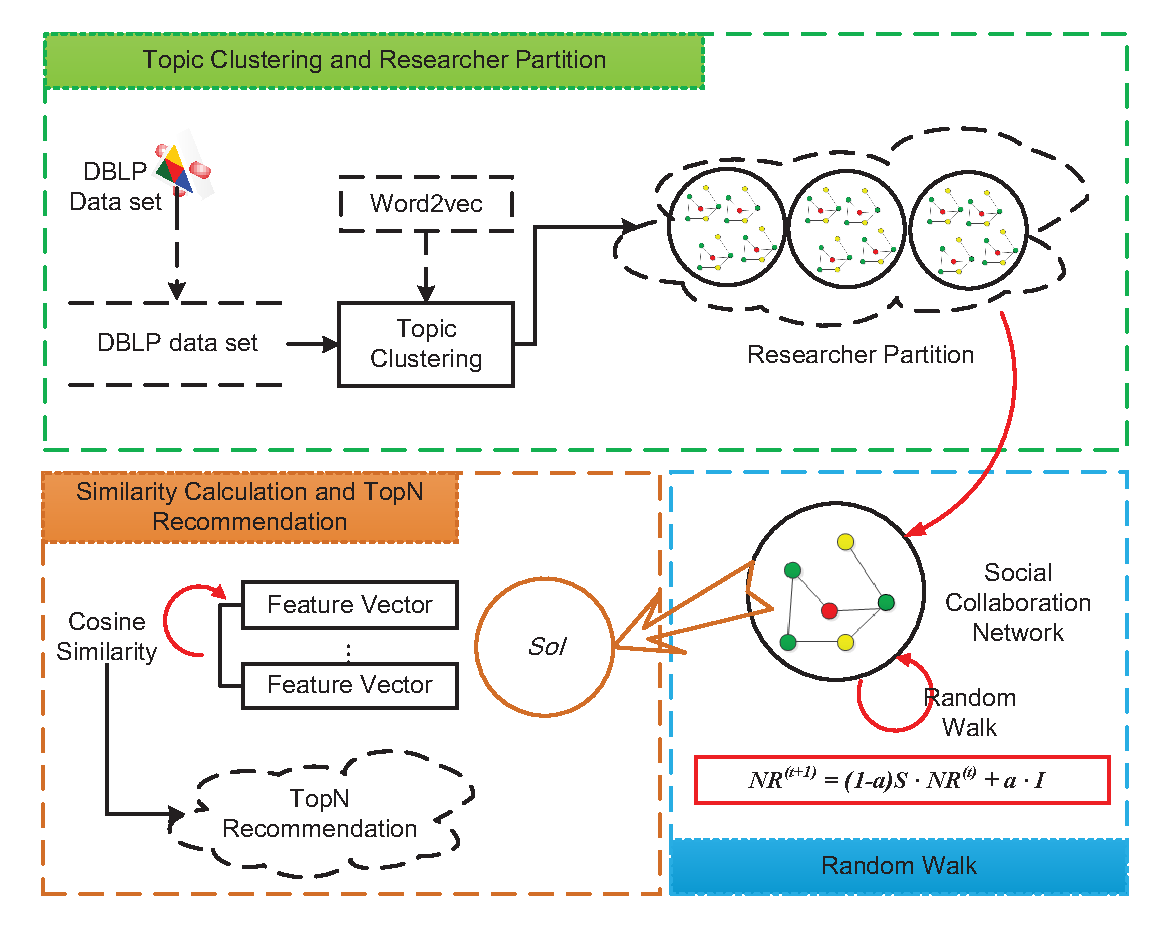
\includegraphics [width=4in]{Fig1.eps}
\end{figure}

\begin{algorithm}[!hbt]
  \captionof{algorithm}{Pseudo-code of the proposed scheme}
  \label{Algorithm1}
  \begin{algorithmic}[1]
  \State $SoI \leftarrow Init()$
  \For {$d$ in $D$} // Traverse domains set $D$.
        \State $\mathbf{S} \leftarrow ComputeTransferMatrix(d)$
        \State $SoI_{d,0}, R, Q \leftarrow InitVec()$
        \For {$k \leftarrow 0$~to~$MaxIteration-1$}
            \State $diff \leftarrow 0$
            \For {$i \leftarrow 0$~ to~$len(Q)-1$}
                \State $SoI_{d,k_{i}} = \alpha\sum_{j=0}^{len(Q)} S_{i,j}SoI_{d,j}+(1-\alpha) Q_{i}$
                \State $diff \leftarrow diff +(SoI_{d,k}-SoI_{d,k-1})$
            \EndFor
            \If {$diff<MinDelta$}
                \BREAK
            \EndIf
        \EndFor
  \EndFor
  \For {$p_{1}$ in $P$}
        \For {$p_{2}$ in $P$}
            \State $Similarity_{p_{1},p_{2}} \leftarrow CosSim(SOI_{p_{1},p_{2}})$
        \EndFor
  \EndFor
  \State RecommendTopN()
  \end{algorithmic}
\end{algorithm}

\subsection*{Topic Clustering and Researcher Partition}
% -----------------------------------------------------------------------------
It is a content-based method for topic clustering and researcher partition, which generates various domains and maps all researchers into these domains. In this section, we work on partitioning researchers according to academic topics. We use a famous tool of Natural Language Processing (NLP) called word2vec~\cite{goldberg2014word2vec} to cluster the  academic topics. There is another well-developed topic clustering method, Latent Dirichlet Allocation (LDA)~\cite{blei2003latent}. LDA mainly generates the probability distribution of words and documents with the input of number of documents. However, the feature of each researcher is represented by several documents (his publications). It is difficult to generate accurate feature description for each researcher, hence it is unsuitable to partition the researchers according to their publications' probability distribution. Word2vec provides an efficient implementation of the continuous of \emph{bag-of-words} and \emph{skip-gram} architectures for computing vector representations of words. It takes a text corpus as the input and produces the word vectors as the output. The final word vector file can be used as features in many NLP and machine learning applications. The word vectors can be also used for deriving word classes from huge data sets. This is achieved by performing K-means clustering on top of the word vectors. The output is a vocabulary file with words and their corresponding domain IDs. In the case of our CCRec model, the input data is a set of titles from all the papers created by each researcher. The titles are split in many sequential words. In addition, it is necessary to filter out some "Stop words"~\footnote{https://code.google.com/p/stop-words/}, e.g. "of", "the", "and", etc. When extracting words from titles, the set of preprocessed words can be used outline the core contents of papers, which are signified as valuable and reliable corpus to denote a variety of academic topics. We run word2vec on this corpus, the word vector can be automatically generated and the K-means clustering method is alternative executed. The output file include all academic words and their corresponding domain IDs. Now that the academic topics are clustered and the words are marked to each topics. We use a matrix $\mathbf{W}$ to denote these mapping relation. If a word $w$ is marked to a topic $d$, $W_{w,d}$ will be $1$, otherwise 0.

In addition, CCRec partitions researchers to specific domains through the following approaches: 1) Extract subject terms from the publications' titles of researcher $s$'s (After filtering out the stop words). We use $words_{s}$ to represent the set of researcher $s$'s subject terms. 2) Traverse all the subject terms in $words_{a}$ and check the matrix $\mathbf{W}$. The model tags the researcher for particular domains that contain these subject terms. We use the matrix $\mathbf{A}$ to denote the relations of researcher and topic. Equation~\ref{matrixA} shows the process of computing the matrix $\mathbf{A}$.

\begin{equation}
\label{matrixA}
A_{s,d}=\left\{\begin{array}{ll}
1 & \exists~ word~ w \in word_{s},~ that~ W_{w,d}=1\\
0 & \forall~ word~ w \in word_{s},~ that~ W_{w,d}\neq 1\\
\end{array}\right.
\end{equation}

According to the equation, if $A_{a,d}=1$, the researcher $a$ is marked to topic $d$. It should be emphasized that one researcher always belongs to several domains and there are also many researchers in one domain. Figure~\ref{Fig. 2} illustrates an example. Assuming that CCRec extracts 12 subject terms from the publications titles of researcher $S1$. After topic clustering, we can see that, three of these subject terms are assigned to domain $A$, seven in $B$, and two in $C$. Thus, researcher $S1$ is tagged for domains $A$, $B$ and $C$. That is, $A_{S1,A},A_{S1,B},A_{S1,C}$ are all equals 1. Through this method, each domain contains numerous researchers.

\begin{figure}[!hbt]
\caption{{\bf Researcher Partition.} Illustrates an example of partition researchers to several domains.}
\label{Fig. 2}
%\center
%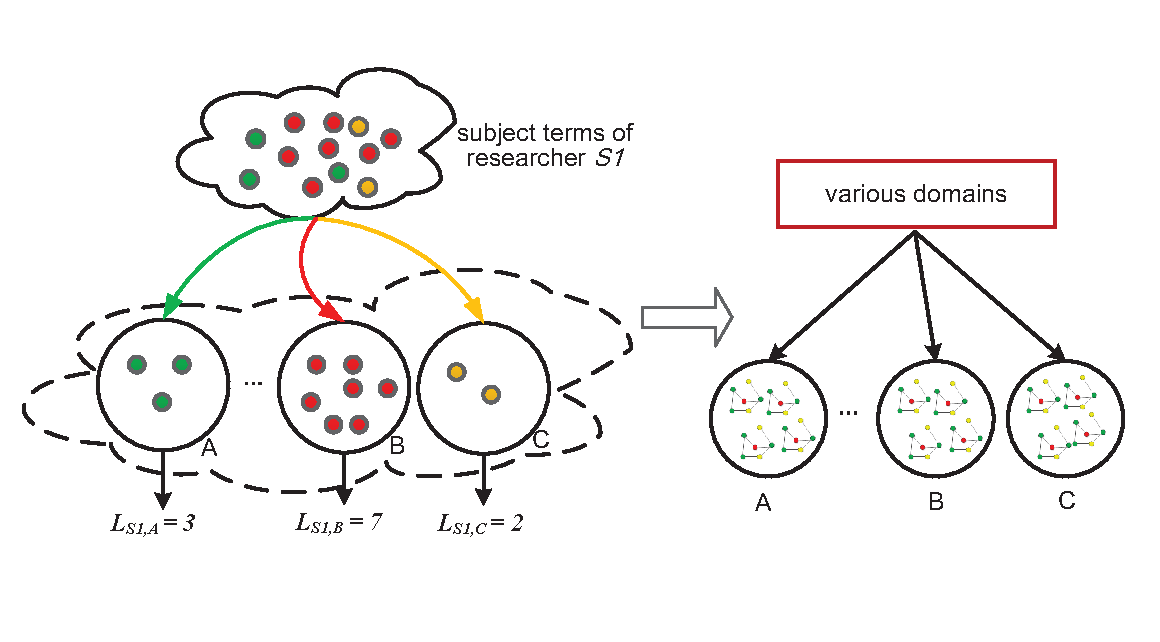
\includegraphics [width=4in]{Fig2.eps}
\end{figure}

\subsection*{Feature Vector Calculation}
% -----------------------------------------------------------------------------
As mentioned in Introduction, in general, researchers devote themselves to several adjacent domains. But in the case of attention and strength of influence in various domains, there are often some biases. To measure the influence of researchers, we define the Strength of Influence ($SoI$) to denote the academic values (Rank Score) of researchers in different domains, which can be regarded as the feature vector elements of researchers. To compute $\emph{SOI}$, we adopt a social-network based model, the random walk with restart model RWR. In RWR, the rank score of a node is determined by the voting contributions from neighbors, which can be reflected by the count of neighbors in addition to the rank score and the out-degree of each neighbor. The rank score in RWR can be used to represent the node importance in a social network. Therefore, we firstly model the social-networks. There are numerous researchers with similar research interests in domain $d$. ($\forall reseachers a, that A_{s,d}=1$) Their co-author relationships are the most obvious and important links among researchers, which can be modeled by a social network $network^d$ for domain $d$. Thus, there are many co-author networks corresponding to different domains. We run the RWR model on $network^d$, the generated rank score of each node in the domain is used to denote academic values, that is $\emph{SOI}$. The core equation of the RWR model is shown in Eq.~(\ref{eq:rwr}) below:
\begin{equation}\label{eq:rwr}
R_{d}^{(t+1)}=\alpha \mathbf{S}R_{d}^{(t)}+(1-\alpha)q
\end{equation}
where $R_{d}$ represents the rank score vector of all researchers in domain $d$, $q$ is the initial vector $R^0$, and $\alpha$ denotes the damping coefficient. In normal random walk model, $\alpha$ takes the value of 0.8, which has been confirmed in our experiments. $\mathbf{S}$ is the transfer matrix, which drives the random walker skipping to next node with a probability. RWR is an iterative process. After limited iterations, the vector $R$ will be convergent. In this scenario, $SOI_{d,s}=R_{d,s}$. That is, the final value of the vector item $R_{d,s}$ is the $SoI$ of researcher $s$ in domain d.

In addition, with the help of RWR, the $SoI$ in various domains is quantified for each researcher. To measure researchers' academic feature, we define the vector $F$ with $SoI$ as $F_{d,s}=SOI_{d,s}$.

\subsection*{Collaboration Recommendation Based on Feature Vector Similarity}
% -----------------------------------------------------------------------------
CCRec recommends collaborators for researchers based on their similarities. To measure the academic feature similarities of researchers, we borrow a standard method, \emph{cosine similarity} (CS), as shown in Eq.~(\ref{eq:cossim}). CS is employed to define the similarity between two users $s_{1}$ and $s_{2}$ based on their feature vectors $F_{s_{1}}$ and $F_{s_{2}}$.
\begin{equation}\label{eq:cossim}
Sim(s_{1},s_{2})=\frac{\sum_{i=1}^{n}(F_{s_{1},i}*F_{s_{2},i})}{\sqrt{\sum_{i=1}^{n}F_{s_{1},i}^2}*\sqrt{\sum_{i=1}^{n}F_{s_{2},i}^2}}
\end{equation}
Finally, we consider that researchers with high similarities have common interests. Therefore, they should be recommended to each other as potential academic collaborators. Hence, CCRec provides a \emph{Top-N} recommendation list for each researcher.

% =============================================================================
\section*{Results}
% =============================================================================
We conduct various experiments using data from DBLP~\cite{Ley:DBLP} from year 2000 to 2014, a computer science bibliography website hosted at University of Trier, Germany, which indexes more than 2.3 million articles on computer science and contains many links to home pages of computer scientists. Each DBLP record contains these attributes, authors, title, pages, years, crossref, proceedings or journals, etc. In a coauthor graph, there are some isolated authors whose publications are without any cooperation. Thus, they nearly have no relationship with other scholars. Furthermore, we define these isolated authors as the weak nodes, since their degree values are 0. It is clear that the weak nodes have little impact on the random walk. Therefore, to measure the performance of CCRec better, we ignore the weak nodes whose degrees are less than 1. We also ignore the problem of author disambiguation and assume that each researcher has an independent name. We extracted the subsets of the entire data using the required information, which are all in the field of data mining involving 34 journals and 49 conferences. The data was modeled by an academic social network, which contains 59659 nodes (authors) and 90282 edges (coauthor relations). In this network, there are authors, relations between authors and the information about their publications, so we can associate these to recommend collaborators. Moreover, as described in Table~\ref{tab:statdblp}, the average degree is 1.531, and the number of the keywords is 104587. We divided the data set into two parts: the data before year 2011 as a training set, and the data after 2011 as a testing set.

\begin{table}[!ht]
\begin{adjustwidth}{-2.25in}{0in}
\caption{\bf{Statistics of Data Set from DBLP}}
\label{tab:statdblp}
\begin{tabular}{|c|c|c|c|}\hline
Nodes&Edges&Average Degree&words\\\hline
59659 &90282 &1.513 &104587\\\hline
\end{tabular}
\end{adjustwidth}
\end{table}

We embarked on benchmarking experiments involving CCRec. To evaluate the performance of CCRec model visually, we employ three popular metrics those are widely used in the recommender systems: \emph{Precision}, \emph{Recall} and \emph{F1}~\cite{shani2011evaluating}. In this academic recommender system, there are a recommendation list, as well as a collaborator list in testing data set. The performance of recommender system can be well reflected by the intersection ratio of the two list. There are four sets comparing the two list. A: recommended and collaborated. B: recommended but not collaborated. C: not recommended but collaborated. D: not recommended and not collaborated.

So, the definition of precision is defined as:
\begin{equation}
\label{equ7}
Precision=\frac{A}{A+B}
\end{equation}

Recall is defined as:
\begin{equation}
\label{equ8}
Recall=\frac{A}{A+C}
\end{equation}

F1 is defined as:
\begin{equation}
\label{equ9}
F1=\frac{2(Precision \ast Recall)}{Precision + Recall}
\end{equation}

We compared CCRec with the following two approaches, which have been proved to be effective in academic collaborators recommendation. ACRec: a random walk recommendation model based on collaboration networks~\cite{li2014acrec}, which uses three academic factors to recommend collaborators based on the RWR. ACRec was demonstrated to do excellently in most valuable collaborators recommendation. CNRec: a common neighbors based recommendation model~\cite{lopes2010collaboration}, which is famous and widely used in social-network based recommendation. ACRec and CNRec can be delegated as the high accurate recommender systems. Three groups of experiments were conducted. 1) Find the MVCs, who may have known each other before, or be active in adjacent circles, 2) Recommend MPCs, who have never cooperated with the target researcher before, 3) Evaluate how domains clustering impact the performance of CCRec. For each experiment, there are 500 domains clustered. we randomly chose 100 constant researchers who are at least somewhat active in academic activities. We generated collaborators recommendation for these 100 researchers, and then computed the average of precision, recall and $F1$. Figures 3 to 6 show the experimental analysis and result. The source data of the figures is in~\nameref{S1_Figures}.

All experiments were performed using a 64-bit Linux-based operation system, Ubuntu 12.04 with a 4-duo and 32GHz Intel CPU, 4-G Bytes memory. All the programs were implemented with Python.

\subsection*{Most Valuable Collaborators Recommendation}
% -----------------------------------------------------------------------------
In our previous work~\cite{li2014acrec}, We proposed an ACRec model which generates the most valuable collaborators recommendation for researchers. In this section, we analyze the performance of CCRec and ACRec in terms of generating the most valuable collaborators recommendation. The comparative results are shown in Figure~\ref{Fig. 3}.

\begin{figure}[!hbt]
\caption{{\bf Performance of CCRec and ACRec on most valuable collaborators recommendation.} The abscissas denote the length of recommendation list. The ordinates respectively represent the values of precision, recall and F1.}
\label{Fig. 3}
%\center
%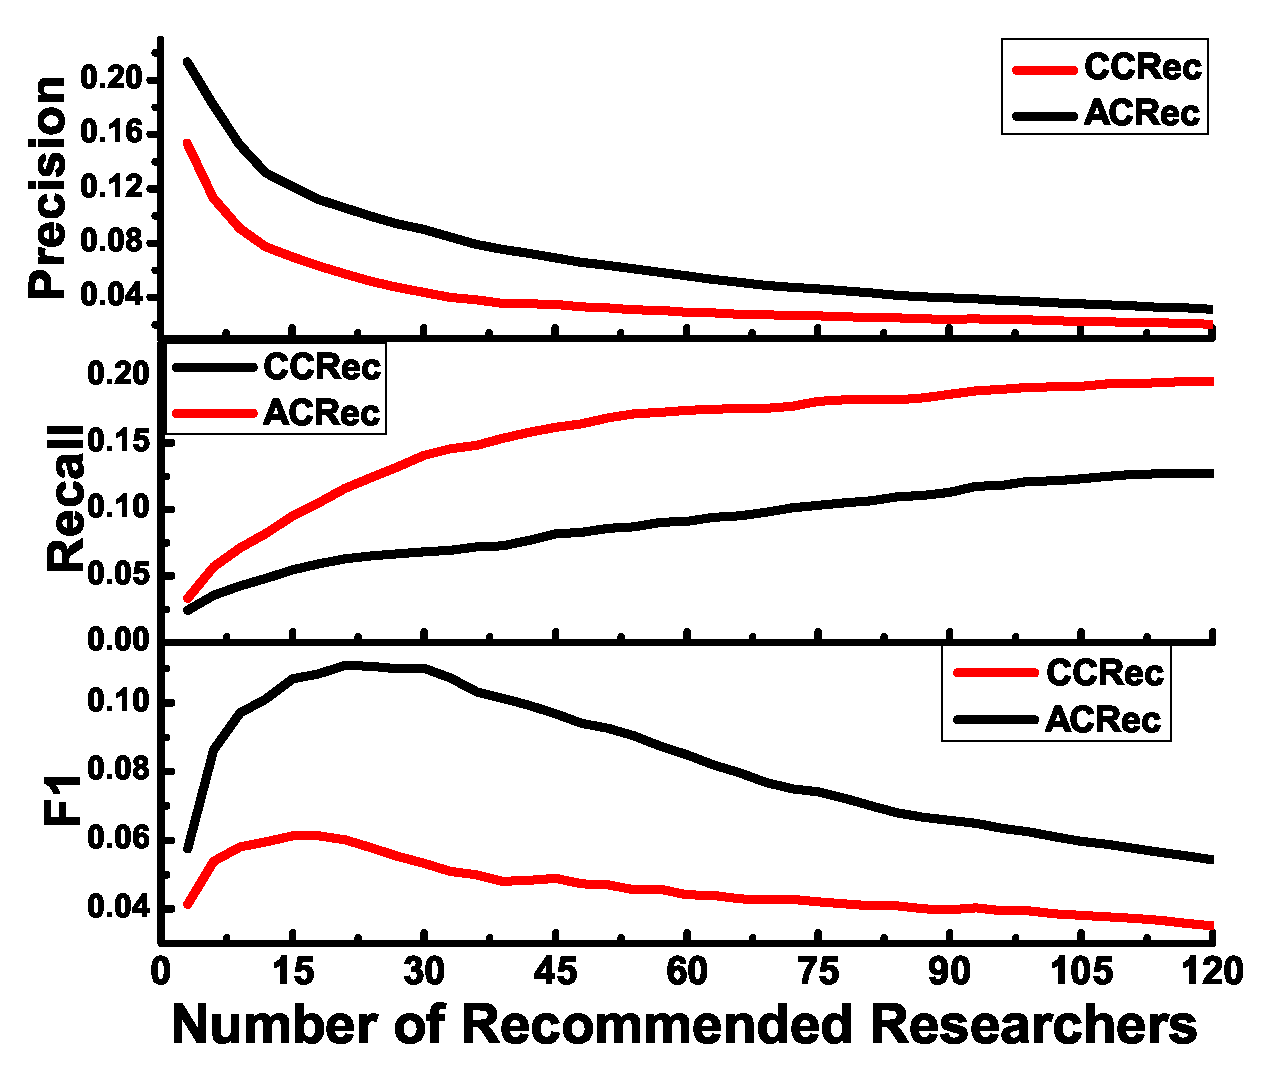
\includegraphics [width=\textwidth]{Fig3.eps}
\end{figure}

As shown in Figure~\ref{Fig. 3}, The number of recommended collaborators has an obvious influence on the metrics with a clear trend. In the case of CCRec, as shown in Figure~\ref{Fig. 3}(A), the precision drops when the number of recommended collaborators is increasing. At the same time, the recall in Figure~\ref{Fig. 3}(B) rises with the increase of recommendation list, which finally approximates to $20\%$. In the case of ACRec, it has the same trend with CCRec in terms of precision and recall. Thus it can be verified that precision and recall are a pair of contradictory metrics. In order to weigh the two metrics to maximize profit, G. Shani et al.~\cite{shani2011evaluating} adopted the metric $F1$. Figure~\ref{Fig. 3}(C) describes the performance of CCRec and ACRec on $F1$. In case of CCRec model, $F1$ generally increases until the number of recommended collaborators is over 15, and then decreases gradually. Since point 15 is exactly the peak of $F1$. We can see that, CCRec performs best when recommending 15 collaborators to each researcher, and the $F1$ can reach $6.13\%$. However, in this scenario, ACRec gets its' highest $F1$ score $11.01\%$ at point 30.

A reflection of Figure~\ref{Fig. 3} substantiates that ACRec outperforms CCRec in terms of generating the most valuable collaborators recommendation. This is because, ACRec is based on the link-importance guiding random walk, which considers the walk distance and rank score and seeks the most valuable collaborators who may have known each other before, or are active in adjacent circles. Thus, there is no obvious superiority for CCRec to find the most valuable collaborators in adjacent circles compared with ACRec. While, the superiority of CCRec lies in recommending MPCs as follows.

\subsection*{Most Potential Collaborators Recommendation}
% -----------------------------------------------------------------------------
We define the Most Potential Collaborators as collaborators who are worthy of being recommended and have never cooperated with the target researcher. Generating recommendations pertaining to the most potential collaborators is of great significance as the new collaborators are more meaningful and practical in the reality of academia. In this section, we explored the performance of CCRec, ACRec and CNRec when recommending the most potential collaborators.

Figure~\ref{Fig. 4} shows the performance of CCRec, ACRec and CNRec in terms of precision, recall and $F1$ with the number of recommended collaborators increasing. It can be observed that CCRec significantly outperforms ACRec and CNRec all the time on these three metrics. CCRec shows a downwards trend for precision and an upwards trend for recall rate. In the case of $F1$, it reaches a peak of $4.18\%$ when recommending 21 researchers. From Figure~\ref{Fig. 4}, it is also evident that in relation to the generation of the most potential collaboration recommendations, ACRec outperforms CCRec in terms of the evaluation metrics we utilized.

\begin{figure}[!hbt]
\caption{{\bf Performance of CCRec, ACRec and CNRec on most potential collaborators recommendation.} The abscissas denote the length of recommendation list. The ordinates respectively represent the values of precision, recall and F1.}
\label{Fig. 4}
%\center
%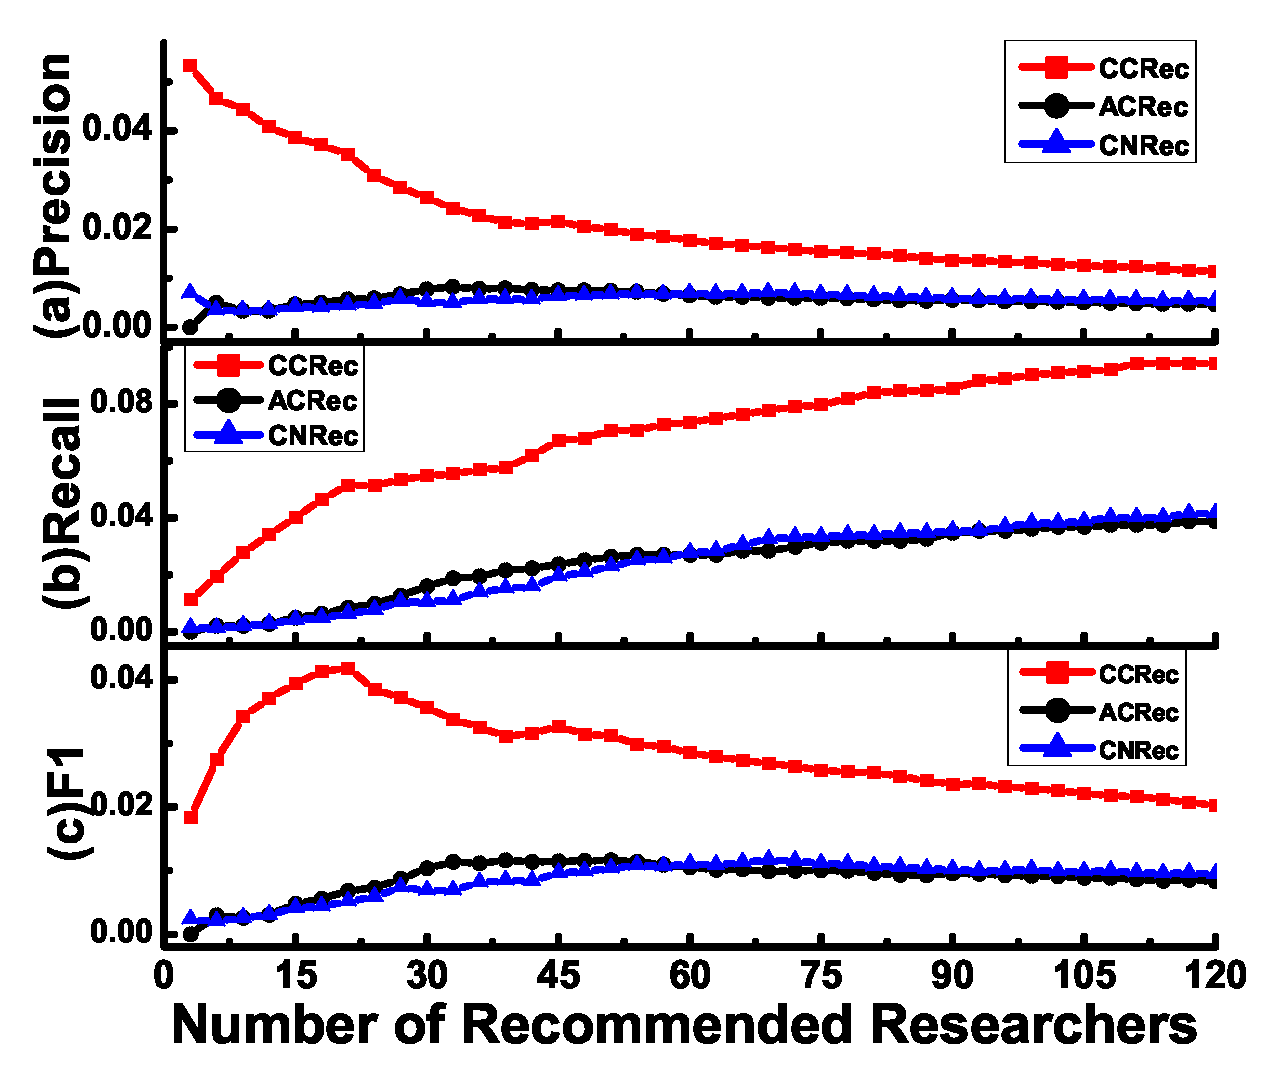
\includegraphics [width=\textwidth]{Fig4.eps}
\end{figure}

Simply, CCRec outperforms ACRec and CNRec with higher precision, recall and $F1$ on making the most potential collaborators. Each researcher is represented by the feature vector, as well as CCRec model which combines publications contents and collaboration networks to define the vector. Such a procedure has distinct advantages (e.g. rich information, more accurately to represent researchers' feature) in recommending new collaborators.

\subsection*{Impact of Clustered Domains Number}
% -----------------------------------------------------------------------------
In this work, we clustered 500 topics based on DBLP data set and matched researchers to different domains. Here we analyzed the statistics of these domains. As described in Figure~\ref{Fig. 5}, in terms of the number of researches in each domain, there are about 56 domains that contain up to 100 researchers, and two domains contain more than 2500 researchers. We can come to conclusion that, various domains show large different in scales. What's more, as shown in Figure~\ref{Fig. 5}(B), most researchers are active in 2 to 20 domains. However, there is no clear standard to make the domains division. The statistics shows inconsistency with different clustering granularity. In this section, we exploit the impact of clustered domains number on the performance of CCRec.

\begin{figure}[!hbt]
\caption{{\bf Statistics of data after topic clustering and researcher partition}}
\label{Fig. 5}
%\center
%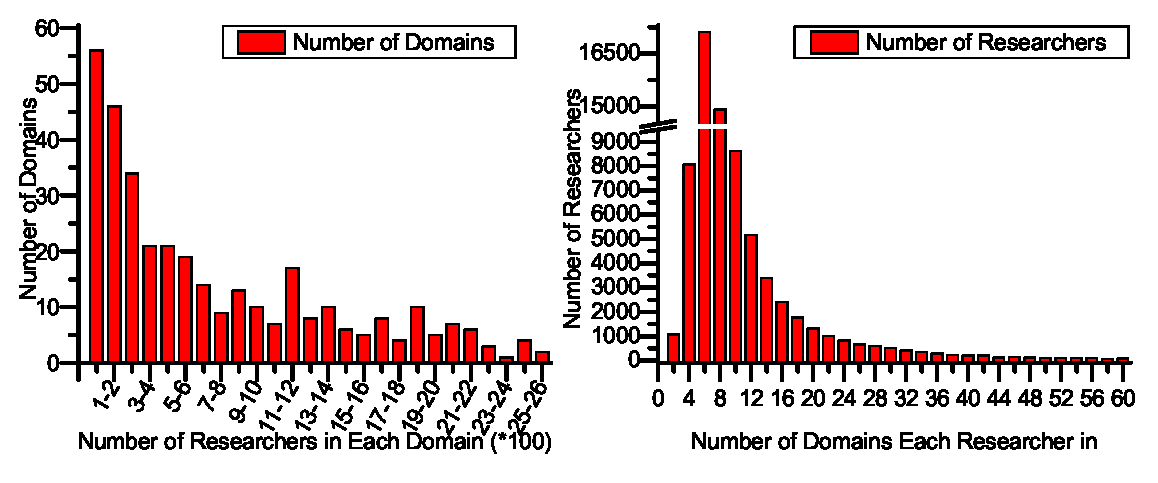
\includegraphics [width=\textwidth]{Fig5.eps}
\end{figure}

We adopted the following experiment settings: (1) Evaluate how the precision, recall and $F1$ score change with the number of collaborators recommended, (2) Generate the most potential collaborators recommendation for those 100 researchers selected above and (3) Recommend 21 potential collaborators for each researcher. Figure~\ref{Fig. 6} shows the experimental results.

\begin{figure}[!hbt]
\caption{{\bf The impact of clustered domains number on CCRec.} The abscissas denote the length of recommendation list. The ordinates respectively represent the values of precision, recall and F1.}
\label{Fig. 6}
%\center
%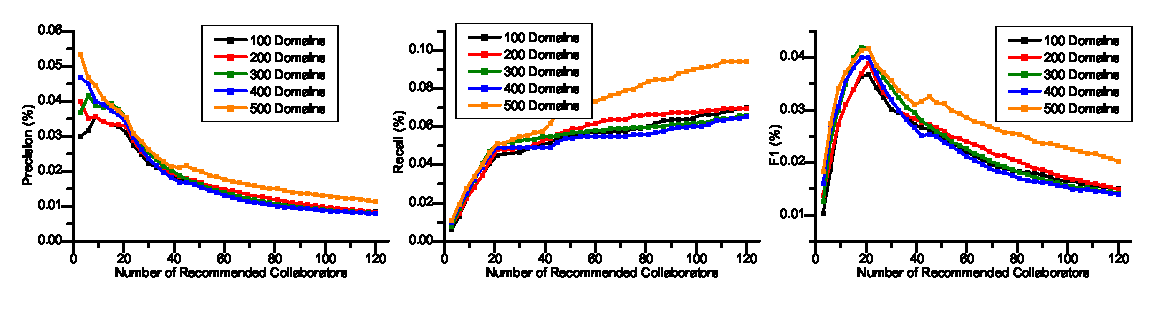
\includegraphics [width=\textwidth]{Fig6.eps}
\end{figure}

According to Figure~\ref{Fig. 6}, the number of clustered domains do have certain effects on the performance of CCRec. If the number of clustered domains is appropriate, the $F1$ score achieves some enhancement. In this situation, when clustering the data mining academia into 500 domains, CCRec performs best over precision, recall and $F1$ score.

In summary, our proposed model, which combines content-based and social network-based methods shows improvement. Furthermore, in terms of precision, recall and $F1$, CCRec outperforms ACRec and CNRec generating the most potential collaborators (MPCs) recommendations for academic researchers.

% =============================================================================
\section*{Conclusions}
% =============================================================================
In this paper, we focused on how to find researchers' MPCs based on big scholarly data which is necessary in current academia. To this end, we proposed a novel recommendation model called CCRec, by combining the features of publications content and collaboration networks. A topic clustering model and a random walk model were adopted to obtain researchers features, and make MPCs recommendation for researchers. We conducted extensive experiments on a subset of DBLP data set to evaluate the performance of CCRec in comparison to other state-of-the-art methods: ACRec and CNRec. Our experimental results show that, CCRec outperforms ACRec and CNRec in terms of precision, recall and $F1$ score. Due the the utilization of a topic clustering model, the problem of topic drift in academic research has been solved to some extent.

Our research on CCRec reveals that the combination of content-based and network-based methods can improve the generation of effective academic collaborations. Nonetheless, there is still room for future study in this direction. We extracted the titles of publications as the corpus of the topic clustering model, which are not more comprehensive than the abstract and main body of publications. Additionally, specific metrics should be utilized to evaluate the impact of topic drift. As future work, more experiments and studies will be conducted.

\section*{Supporting Information}

% Include only the SI item label in the subsection heading. Use the \nameref{label} command to cite SI items in the text.
\subsection*{S1 Figure}
\label{S1_Figures}
{\bf The source data of figures from 3 to 6.}

% Do NOT remove this, even if you are not including acknowledgments.
%\section*{Acknowledgments}

\nolinenumbers

%\section*{References}
% Either type in your references using
% \begin{thebibliography}{}
% \bibitem{}
% Text
% \end{thebibliography}
%
% OR
%
% Compile your BiBTeX database using our plos2009.bst
% style file and paste the contents of your .bbl file
% here.
%

\begin{thebibliography}{10}
\providecommand{\url}[1]{\texttt{#1}}
\providecommand{\urlprefix}{URL }
\expandafter\ifx\csname urlstyle\endcsname\relax
  \providecommand{\doi}[1]{doi:\discretionary{}{}{}#1}\else
  \providecommand{\doi}{doi:\discretionary{}{}{}\begingroup
  \urlstyle{rm}\Url}\fi
\providecommand{\bibAnnoteFile}[1]{%
  \IfFileExists{#1}{\begin{quotation}\noindent\textsc{Key:} #1\\
  \textsc{Annotation:}\ \input{#1}\end{quotation}}{}}
\providecommand{\bibAnnote}[2]{%
  \begin{quotation}\noindent\textsc{Key:} #1\\
  \textsc{Annotation:}\ #2\end{quotation}}
\providecommand{\eprint}[2][]{\url{#2}}

\bibitem{lee2005impact}
Lee S, Bozeman B (2005) The impact of research collaboration on scientific
  productivity.
\newblock Soc Stud Sci 35: 673--702.
\bibAnnoteFile{lee2005impact}

\bibitem{lopes2010collaboration}
Lopes GR, Moro MM, Wives LK, De~Oliveira JPM (2010) Collaboration
  recommendation on academic social networks.
\newblock In: Advances in Conceptual Modeling--Applications and Challenges,
  Springer. pp. 190--199.
\bibAnnoteFile{lopes2010collaboration}

\bibitem{chen2009make}
Chen J, Geyer W, Dugan C, Muller M, Guy I (2009) Make new friends, but keep the
  old: recommending people on social networking sites.
\newblock In: Proc. SIGCHI. pp. 201--210.
\bibAnnoteFile{chen2009make}

\bibitem{dimicco2008motivations}
DiMicco J, Millen DR, Geyer W, Dugan C, Brownholtz B, et~al. (2008) Motivations
  for social networking at work.
\newblock In: Proce. ACM CSCW. pp. 711--720.
\bibAnnoteFile{dimicco2008motivations}

\bibitem{li2014acrec}
Li J, Xia F, Wang W, Chen Z, Asabere NY, et~al. (2014) Acrec: a co-authorship
  based random walk model for academic collaboration recommendation.
\newblock In: Proc. WWW. pp. 1209--1214.
\bibAnnoteFile{li2014acrec}

\bibitem{xia2014mvcwalker}
Xia F, Chen Z, Wang W, Li J, Yang LT (2014) Mvcwalker: Random walk based most
  valuable collaborators recommendation exploiting academic factors.
\newblock IEEE Trans Emerg Top Comput 2: 364-375.
\bibAnnoteFile{xia2014mvcwalker}

\bibitem{gollapalli2012similar}
Gollapalli SD, Mitra P, Giles CL (2012) Similar researcher search in academic
  environments.
\newblock In: Proc. ACM/IEEE JCDL. pp. 167--170.
\bibAnnoteFile{gollapalli2012similar}

\bibitem{kim2010collaborative}
Kim HN, Ji AT, Ha I, Jo GS (2010) Collaborative filtering based on
  collaborative tagging for enhancing the quality of recommendation.
\newblock Electron Commer Res Appl 9: 73--83.
\bibAnnoteFile{kim2010collaborative}

\bibitem{tang2012cross}
Tang J, Wu S, Sun J, Su H (2012) Cross-domain collaboration recommendation.
\newblock In: Proc. SIGKDD. pp. 1285--1293.
\bibAnnoteFile{tang2012cross}

\bibitem{ma2011recommender}
Ma H, Zhou D, Liu C, Lyu MR, King I (2011) Recommender systems with social
  regularization.
\newblock In: Proc.ACM WSDM. pp. 287--296.
\bibAnnoteFile{ma2011recommender}

\bibitem{huynh2013trend}
Huynh T, Hoang K, Lam D (2013) Trend based vertex similarity for academic
  collaboration recommendation.
\newblock In: Computational Collective Intelligence. Technologies and
  Applications, Springer. pp. 11--20.
\bibAnnoteFile{huynh2013trend}

\bibitem{chen2012discovering}
Chen HH, Gou L, Zhang XL, Giles CL (2012) Discovering missing links in networks
  using vertex similarity measures.
\newblock In: Proc. ACM SAC. pp. 138--143.
\bibAnnoteFile{chen2012discovering}

\bibitem{sun2011co}
Sun Y, Barber R, Gupta M, Aggarwal CC, Han J (2011) Co-author relationship
  prediction in heterogeneous bibliographic networks.
\newblock In: ASONAM. IEEE, pp. 121--128.
\bibAnnoteFile{sun2011co}

\bibitem{lichtenwalter2010new}
Lichtenwalter RN, Lussier JT, Chawla NV (2010) New perspectives and methods in
  link prediction.
\newblock In: Proc. SIGKDD. pp. 243--252.
\bibAnnoteFile{lichtenwalter2010new}

\bibitem{lee2011recommending}
Lee DH, Brusilovsky P, Schleyer T (2011) Recommending collaborators using
  social features and mesh terms.
\newblock Proceedings of the American Society for Information Science and
  Technology 48: 1--10.
\bibAnnoteFile{lee2011recommending}

\bibitem{cohen2013recommending}
Cohen S, Ebel L (2013) Recommending collaborators using keywords.
\newblock In: Proc. WWW. pp. 959--962.
\bibAnnoteFile{cohen2013recommending}

\bibitem{petertonkoker2014scientific}
Petertonkoker J, Reinhardt W, Surve J, Sureka P (2014) Scientific
  recommendations to enhance scholarly awareness and foster collaboration.
\newblock In: Recommender Systems for Technology Enhanced Learning, Springer.
  pp. 283--306.
\bibAnnoteFile{petertonkoker2014scientific}

\bibitem{xia2014socially}
Xia F, Asabere NY, Liu H, Chen Z, Wang W (2014) Socially aware conference
  participant recommendation with personality traits.
\newblock IEEE Systems Journal .
\bibAnnoteFile{xia2014socially}

\bibitem{chaiwanarom2014collaborator}
Chaiwanarom P, Lursinsap C (2014) Collaborator recommendation in
  interdisciplinary computer science using degrees of collaborative forces,
  temporal evolution of research interest, and comparative seniority status.
\newblock Knowledge-Based Systems .
\bibAnnoteFile{chaiwanarom2014collaborator}

\bibitem{chen2011collabseer}
Chen HH, Gou L, Zhang X, Giles CL (2011) Collabseer: a search engine for
  collaboration discovery.
\newblock In: Proc. ACM/IEEE JCDL. pp. 231--240.
\bibAnnoteFile{chen2011collabseer}

\bibitem{li2014author}
Li C, Cheung WK, Ye Y, Zhang X, Chu D, et~al. (2014) The author-topic-community
  model for author interest profiling and community discovery.
\newblock Knowledge and Information Systems : 1--25.
\bibAnnoteFile{li2014author}

\bibitem{goldberg2014word2vec}
Goldberg Y, Levy O (2014) word2vec explained: deriving mikolov et al.'s
  negative-sampling word-embedding method.
\newblock arXiv preprint arXiv:14023722 .
\bibAnnoteFile{goldberg2014word2vec}

\bibitem{blei2003latent}
Blei DM, Ng AY, Jordan MI (2003) Latent dirichlet allocation.
\newblock the Journal of machine Learning research 3: 993--1022.
\bibAnnoteFile{blei2003latent}

\bibitem{Ley:DBLP}
Ley M (2009) Dblp: some lessons learned.
\newblock Proceedings VLDB Endowment 2: 1493-1500.
\bibAnnoteFile{Ley:DBLP}

\bibitem{shani2011evaluating}
Shani G, Gunawardana A (2011) Evaluating recommendation systems.
\newblock In: Recommender systems handbook, Springer. pp. 257--297.
\bibAnnoteFile{shani2011evaluating}

\end{thebibliography}


%\bibliography{CCRec}

\end{document}

